\onehalfspacing
\section{Đề số 13}
\graphicspath{{./img/}}
\begin{bt} 
    \hfill
	\begin{enumerate}[a.]
		\item $\left|x+\frac{1}{5}\right|-4=-2$
        \item $2 x-\frac{1}{5}=\frac{6}{5} x-\frac{1}{2}$
        \item $(x-3)^{x+2}-(x-3)^{x+8}=0$
	\end{enumerate}
	\loigiai{
        \begin{enumerate}
            \item Ta có:\\
            $\left|x+\frac{1}{5}\right|-4=-2 \Leftrightarrow\left|x+\frac{1}{5}\right|=2 \Leftrightarrow {\left[\begin{array} { l } 
            { x + \frac { 1 } { 5 } = 2 } \\
            { x + \frac { 1 } { 5 } = - 2 }
            \end{array} \Leftrightarrow \left[\begin{array}{l}
            x=\frac{9}{5} \\
            x=-\frac{11}{5}
            \end{array}\right.\right.} \\
            \text {Vậy với } x=\frac{9}{5} \text { hoặc } x=-\frac{11}{5} \text { thì }\left|x+\frac{1}{5}\right|-4=-2$
            \item Ta có:
            $
            2 x-\frac{1}{5}=\frac{6}{5} x-\frac{1}{2} \Leftrightarrow \frac{4}{5} x=-\frac{3}{10} \Rightarrow x=-\frac{3}{8}
            $
            \item Ta có: $(x-3)^{x+2}-(x-3)^{x+8}=0 \Leftrightarrow(x-3)^{x+2}\left[1-(x-3)^6\right]=0$
            $\\
            \Leftrightarrow\left[\begin{array} { l } 
            { x - 3 = 0 } \\
            { ( x - 3 ) ^ { 6 } = 1 }
            \end{array} \Leftrightarrow \left[\begin{array}{l}
            x=3 \\
            x=4 \\
            x=2
            \end{array}\right.\right.
            $
        \end{enumerate}
    } 
\end{bt}

\begin{bt}
	Tìm $x, y, z$ biết $\frac{x}{2}=\frac{y}{3}=\frac{z}{4}$ và $x^2+y^2+z^2=116$
	\loigiai{
            $\frac{x}{2}=\frac{y}{3}=\frac{z}{4} \Rightarrow \frac{x^2}{4}=\frac{y^2}{9}=\frac{z^2}{16}=\frac{x^2+y^2+z^2}{4+9+16}=\frac{116}{29}=4 \\[10pt]
            \Rightarrow \frac{x^2}{4}=\frac{y^2}{9}=\frac{z^2}{16}=4 \Rightarrow \frac{x}{2}=\frac{y}{3}=\frac{z}{4}= \pm 2 \\[10pt]
            \text {Vậy }(x ; y ; z)=(4 ; 6 ; 8) \text { hoặc }(x ; y ; z)=(-4 ;-6 ;-8)$
    } 
\end{bt}

\begin{bt}
	Trong vòng bán kết giải bóng đá của trường THCS Phù Đổng có 4 đội thi đấu, gọi $\mathrm{A}$ là tập hợp các cầu thủ; B là tập hợp các số áo thi đấu. Quy tắc mỗi cầu thủ ứng với số áo của họ có phải là một hàm số không? Vì sao?
	\loigiai{
        Quy tắc mỗi cầu thủ ứng với số áo của họ không là một hàm số vì đại lượng cầu thủ không phải là các giá trị bằng số. (trả lời đúng giải thích sai không có điểm)
    }
\end{bt}

\begin{bt}
    Tính giá trị của đa thức $\mathrm{P}=x^3+x^2 y-2 x^2-x y-y^2+3 y+x+2017$ với
    $
    x+y=2
    $
\loigiai{
        $P=x^3+x^2 y-2 x^2-x y-y^2+3 y+x+2017 \\[7pt]
        =x^2(x+y)-2 x^2-y(x+y)+3 y+x+2017 \\[7pt]
        =2 x^2-2 x^2-2 y+3 y+x+2017=x+y+2017=2019 \\[7pt]
        \text {Vậy với } x+y=2 \text { thì } P=2019\\[7pt]
        \text { Hoặc nhóm để xuất hiện } \mathrm{x}+\mathrm{y} \text { - } 2$
}
\end{bt}

\begin{bt}
    Cho : $\frac{3 x-2 y}{4}=\frac{2 z-4 x}{3}=\frac{4 y-3 z}{2}$. Chứng minh: $\frac{x}{2}=\frac{y}{3}=\frac{z}{4}$
\loigiai{
        $\frac{3 x-2 y}{4}=\frac{2 z-4 x}{3}=\frac{4 y-3 z}{2} \\[7pt]
        \Rightarrow \frac{12 x-8 y}{16}=\frac{6 z-12 x}{9}=\frac{8 y-6 z}{4}=\frac{12 x-8 y+6 z-12 x+8 y-6 z}{16+9+4}=0 \\[7pt]
        \Rightarrow 12 x=8 y=6 z \Rightarrow \frac{12 x}{24}=\frac{8 y}{24}=\frac{6 z}{24} \\[7pt]
        \Rightarrow \frac{x}{2}=\frac{y}{3}=\frac{z}{4}$
}
\end{bt}

\begin{bt}
    Tìm các số tự nhiên $\mathrm{x}$, $y$ thỏa mãn: $2 \mathrm{x}^2+3 \mathrm{y}^2=77$  
\loigiai{
    $2 x^2+3 y^2=77 \Rightarrow 3 y^2=77-2 y^2 \leq 77 \Rightarrow y^2 \leq 77 / 3 \Rightarrow y^2 \leq 25$\\[6pt]
    Mà $2 x^2$ chẵn; 77 lẻ $\Rightarrow 3 y^2$ lẻ $\Rightarrow y^2$ lẻ $\Rightarrow y^2 \in\{1 ; 9 ; 25\}$\\[6pt]
    $+y^2=1 \Rightarrow 2 x^2=77-3=74 \Rightarrow x^2=37 \Rightarrow \text { không có số tự nhiên } \mathrm{x} \\[6pt]
    +y^2=9 \Rightarrow 2 x^2=77-27=50 \Rightarrow x^2=25 \Rightarrow x=5 \text { và } y=3 \\[6pt]
    +y^2=25 \Rightarrow 2 x^2=77-75=2 \Rightarrow x^2=1 \Rightarrow x=1 \text { và } y=5$\\[6pt]
    Vậy số tự nhiên $x$, $y$ thỏa mãn $2 x^2+3 y^2=77$ là $(x ; y)=(5 ; 3) ;(1 ; 5)$\\[6pt]
    Học sinh lân lượt thư chọn các số tụ nhiên $x$ (hoặc y) từ $0,1,2, \ldots$ để có được KQ sẽ không được điểm vì không thể hiện được năng lực tu duy số học.
}
\end{bt}

\begin{bt}
    Cho $\triangle \mathrm{ABC}$, tia phân giác của góc $\mathrm{A}$ cắt $\mathrm{BC}$ tại $\mathrm{D}$. Biết $\mathrm{ADB}=85^{\circ}$
    \begin{enumerate}
        \item Tính: $\mathrm{B}-\mathrm{C}$
        \item Tính các góc của $\triangle \mathrm{ABC}$ nếu $4 . B=5 . C$
    \end{enumerate}
\loigiai{
    $$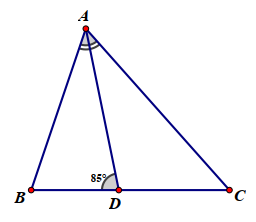
\includegraphics[width=0.4\textwidth]{13-4-lg.png}$$
    \begin{enumerate}
        \item Xét $\triangle \mathrm{ADC}$ có $\mathrm{ADB}$ là góc ngoài tại $\mathrm{D}$\\[5pt]
        $\Rightarrow \mathrm{ADB}=\mathrm{C}+\mathrm{DAC}=85^{\circ}$\\[5pt]
        Xét $\triangle \mathrm{ADB}$ có $\mathrm{ADC}$ là góc ngoài tại $\mathrm{D}$
        $\Rightarrow \mathrm{ADC}=\mathrm{B}+\mathrm{BAD}=180^{\circ}-85^{\circ}=95^{\circ}$\\[5pt]
        Mà $\mathrm{DAC}=\mathrm{BAD}(\mathrm{Vi} \mathrm{AD}$ là tia phân giác của góc $\mathrm{A})$\\[5pt] 
        $\Rightarrow$ Từ $(1)$ và $(2) \Rightarrow \mathrm{B}-\mathrm{C}=95^{\circ}-85^{\circ}=10^{\circ}$
        \item Vì $\mathrm{B}-\mathrm{C}=10^{\circ}$ mà $4 \cdot \mathrm{B}=5 \cdot \mathrm{C} \Rightarrow \frac{\mathrm{B}}{5}=\frac{\mathrm{C}}{4}=\frac{\mathrm{B}-\mathrm{C}}{5-4}=10^{\circ}$\\[5pt] 
        $\Rightarrow B=50^{\circ}$ và $C=40^{\circ} \Rightarrow A=90^{\circ}$
    \end{enumerate}
}
\end{bt}

\begin{bt}
    Cho $\triangle \mathrm{ABC}$ có ba góc nhọn, trung tuyến $\mathrm{AM}$. Trên nửa mặt phẳng bờ $\mathrm{AB}$ chứa điểm $\mathrm{C}$, vẽ đoạn thẳng $\mathrm{AE}$ vuông góc và bằng $\mathrm{AB}$. Trên nửa mặt phẳng bờ $\mathrm{AC}$ chứa điểm $B$, vẽ đoạn thẳng $A D$ vuông góc và bằng $A C$.

\begin{enumerate}
    \item Chứng minh: $\mathrm{BD}=\mathrm{CE}$
    \item Trên tia đối của tia MA lấy $\mathrm{N}$ sao cho $\mathrm{MN}=\mathrm{MA}$. Chứng minh: $\triangle \mathrm{ADE}=\Delta \mathrm{CAN}$.
    \item Gọi I là giao điểm của $\mathrm{DE}$ và $\mathrm{AM}$. Chứng minh: $\frac{\mathrm{AD}^2+\mathrm{IE}^2}{\mathrm{DI}^2+\mathrm{AE}^2}=1$
\end{enumerate}
\loigiai{
    $$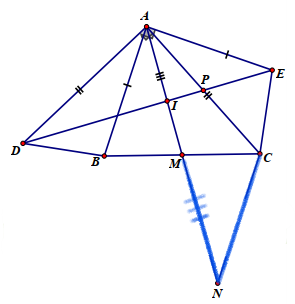
\includegraphics[width=0.4\textwidth]{13-5-lg.png}$$
    \begin{enumerate}
        \item Xét $\triangle \mathrm{ABD}$ và $\triangle \mathrm{ACE}$ có:\\[5pt]
        $\mathrm{AD}=\mathrm{AC}(\mathrm{gt}) \\[5pt]
        \mathrm{AE}=\mathrm{AB}(\mathrm{gt})$ \\[5pt]
        $\mathrm{BAD}=\mathrm{CAE}$ (Cùng phụ với $\mathrm{BAC}$ )\\[5pt] 
        $\Rightarrow \triangle \mathrm{ABD}=\triangle \mathrm{AEC} \text { (c.g.c) } \\[5pt]
        \Rightarrow \mathrm{BD}=\mathrm{CE} \text { (Hai cạnh tương ứng) }$
        \item Xét $\triangle \mathrm{ABM}$ và $\triangle \mathrm{NCM}$ có $\mathrm{AM}=\mathrm{MN}$ (gt); $\mathrm{BM}=\mathrm{CM}$ (gt) $\mathrm{AMB}=\mathrm{AMC}$
        (đối đỉnh)\\[5pt]
        $\Rightarrow \triangle \mathrm{ABM}=\Delta \mathrm{NCM}$ (c.g.c)\\[5pt] 
        $\Rightarrow \mathrm{AB}=\mathrm{CN}$ (hai cạnh tương ứng), $A B M=N C M$ (Hai góc tương ứng)\\[4pt]
        Ta có $\mathrm{ACN}=\mathrm{ACB}+\mathrm{BCN}=\mathrm{ACB}+\mathrm{ABC}=180^{\circ}-\mathrm{BAC}$\\[4pt]
        Lại có $\mathrm{DAE}=\mathrm{DAC}+\mathrm{BAE}-\mathrm{BAC}=180^{\circ}-\mathrm{BAC}$\\[5pt]
        $\Rightarrow \mathrm{DAE}=\mathrm{ACN}$\\[4pt]
        Xét $\triangle \mathrm{ADE}$ và $\triangle \mathrm{ACN}$ có $\mathrm{CN}=\mathrm{AE}$ (cùng bằng $\mathrm{AB}$ )\\[5pt]
        $\mathrm{AC}=\mathrm{AD}(\mathrm{gt})$
        $\mathrm{DAE}=\mathrm{ACN} (\mathrm{cmt}) \\[4pt]
        \Rightarrow \triangle \mathrm{ADE}=\triangle \mathrm{CAN} \text { (c.g.c) }$
        \item  $\text{Vì } \triangle \mathrm{ADE}=\Delta \mathrm{CAN}(\mathrm{cmt}) \Rightarrow \mathrm{NAC}=\mathrm{ADE}$ (Hai góc tương ứng)\\[5pt]
        Gọi $P$ là giao điểm của $\mathrm{DE}$ và $\mathrm{AC}$\\[5pt]
        Xét $\triangle \mathrm{ADP}$ vuông tại $\mathrm{A} \Rightarrow \mathrm{ADE}+\mathrm{APD}=90^{\circ} \Rightarrow \mathrm{NAC}+\mathrm{APD}=90^{\circ}$ $\Rightarrow \mathrm{AI} \perp \mathrm{DE}$\\[5pt]
        Xét $\triangle \mathrm{ADI}$ vuông tại I. Theo ĐL Pytago ta có $\mathrm{AD}^2=\mathrm{DI}^2+\mathrm{AI}^2 \Rightarrow \mathrm{AI}^2=\mathrm{AD}^2-\mathrm{DI}^2$\\[5pt] Xét $\triangle \mathrm{AIE}$ vuông tại I. Theo ĐL Pytago ta có $\mathrm{AE}^2=\mathrm{AI}^2+\mathrm{IE}^2 \Rightarrow \mathrm{AI}^2=\mathrm{AE}^2-\mathrm{IE}^2$\\[5pt] $\Rightarrow \mathrm{AD}^2-\mathrm{DI}^2=\mathrm{AE}^2-\mathrm{IE}^2 \Rightarrow \mathrm{AD}^2+\mathrm{IE}^2=\mathrm{DI}^2+\mathrm{AE}^2 \Rightarrow \frac{\mathrm{AD}^2+\mathrm{IE}^2}{\mathrm{DI}^2+\mathrm{AE}^2}=1$(đpcm)
    \end{enumerate}
}
\end{bt}